\textbf{Ejemplo 5}\\

Dadas las alternativas A, B y C determinar la mejor alternativa usando el método de la TIRI
suponiendo que la TMAR= 25\% pmv, compruebe el resultado usando el VPN. Las inversiones iniciales y el costo anual de operación (CAO) son: \\

\begin{center}
	\begin{tabular}{|p{3.325cm}|p{3.325cm}| p{3.325cm}| p{3.325cm}|}
		\hline
		\begin{tabular}[c]{@{}c@{}}\textbf{Proyecto}\end{tabular} & \begin{tabular}[c]{@{}c@{}}\textbf{A} \end{tabular} & \begin{tabular}[c]{@{}c@{}}\textbf{B} \end{tabular} & \begin{tabular}[c]{@{}c@{}}\textbf{C} \end{tabular} \\ \hline

		Costo                                                     & 100.000  COP                                        & 120.000  COP                                        & 110.000  COP                                        \\ \hline

		CAO año 1                                                 & 10.000  COP                                         & 2.000    COP                                        & 5.500   COP                                         \\ \hline

		CAO año 2                                                 & 12.000  COP                                         & 3.000    COP                                        & 6.000    COP                                        \\ \hline

		CAO año 3                                                 & 14.000  COP                                         & 4.000    COP                                        & 7.000    COP                                        \\ \hline

		CAO año 4                                                 & 16.000   COP                                        & 5.000    COP                                        & 8.500    COP                                        \\ \hline
	\end{tabular}
\end{center}

\textbf{Solución:}\\
%La tabla ira centrada
\begin{center}
	\renewcommand{\arraystretch}{1.5}% Margenes de las celdas
	%Creación de la cuadricula de 3 columnas
	\begin{longtable}[H]{|c|c|c|}
		%Creamos una linea horizontal
		\hline
		%Definimos el color de la primera fila
		\rowcolor[HTML]{FFB183}
		%%%%% INICIO ASIGNACIÓN PERÍODO FOCAL %%%%%%%
		%%%%%%%%%% INICIO TITULO
		%Lo que se hace aquí es mezclar las 3 columnas en una sola
		\multicolumn{3}{|c|}{\cellcolor[HTML]{FFB183}\textbf{1. Asignación período focal}}                                  \\ \hline
		%%%%%%%%%% FIN TITULO
		%%%%% INICIO DECLARACIÓN DE VARIABLES %%%%%%%
		\multicolumn{3}{|c|}{$pf : 0 pmv$}                                                                                  \\ \hline

		%%%%%%%%%%% INICIO TITULO
		\rowcolor[HTML]{FFB183}
		\multicolumn{3}{|c|}{\cellcolor[HTML]{FFB183}\textbf{2. Declaración de variables}}                                  \\ \hline
		\multicolumn{1}{|c|}{\cellcolor[HTML]{FFB183}\textbf{Valores monetarios}} & \multicolumn{1}{c|}{\cellcolor[HTML]{FFB183}\textbf{Valores no monetarios}} & \multicolumn{1}{c|}{\cellcolor[HTML]{FFB183}\textbf{Incógnitas}} \\ \hline
		%%%%%%%%%%% FIN TITULO
		%%%%%%%%%%% INICIO MATEMÁTICAS

		$ \text{Inversión inicial} =   $ $ 20\text{.}000\text{ } COP $ & $ n = 5 pmv $ & $\text{i} = $ $?\text{ } COP$\\
		$ \text{Periodo 1 ingreso} = $ $8\text{.}000\text{ } COP $     & & $ VPN(A)=  ? \text{  } COP $\\
		$ \text{Periodo 2 ingreso} =  $ $ 9\text{.}000\text{ } COP $   & & $ VPN(B)= ?\text{  } COP   $\\
		$ \text{Periodo 3 ingreso} =   $ $ 10\text{.}000\text{ } COP $ & & $ VPN(C)=   ?\text{  } COP $\\
		$ \text{Periodo 4 ingreso} =   $ $ 11\text{.}000\text{ } COP $ & & \\
		\hline
		%%%%%%%%%% FIN MATEMÁTICAS
		%%%%% INICIO FLUJO DE CAJA
		\rowcolor[HTML]{FFB183}
		\multicolumn{3}{|c|}{\cellcolor[HTML]{FFB183}\textbf{3. Diagrama de flujo de caja}}                                 \\ \hline
		%Mezclamos 3 columnas y pondremos el dibujo
		%%%%%%%%%%%%% INSERCIÓN DE LA IMAGEN
		%Deberán descargar las imágenes respectivas del drive y pegarlas en la carpeta
		%n_capitulo/img/ejemplos/1/capitulo1ejemplo1.pdf  (el /1/ es el numero del ejemplo)
		\multicolumn{3}{|c|}{ 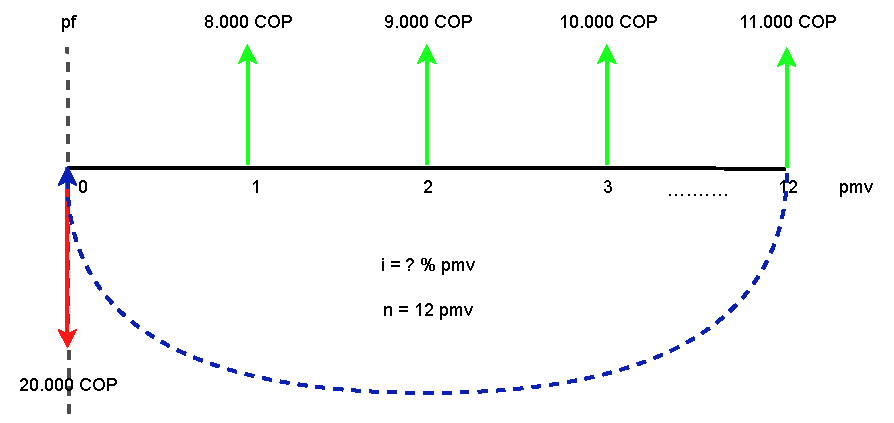
\includegraphics[scale=0.8, trim=0cm -0.5cm 0.0cm -0.5cm]{ejemplos/5/Graf1Ej5Cap11.pdf} }                                              \\\hline
		%%%%%%%%%%%%% FIN INSERCIÓN DE IMAGEN
		%%%%%FIN FLUJO DE CAJA



		%%%%% INICIO DECLARACIÓN FORMULAS
		%%%%%%%%%%% INICIO TITULO
		\rowcolor[HTML]{FFB183}
		\multicolumn{3}{|c|}{\cellcolor[HTML]{FFB183}\textbf{4. Declaración de fórmulas}}                                   \\ \hline
		%%%%%%%%%%% FIN TITULO
		%%%%%%%%%%% INICIO MATEMÁTICAS
		\multicolumn{3}{|c|} {VPN =	$\sum F_{n}(1+i)^{-n}$   Valor presente neto.}                                          \\
		\multicolumn{3}{|c|} {i  $=j/m$ tasa periodica. }                                                                    \\
		\hline

		%%%%%%%%%% FIN MATEMÁTICAS
		%%%%%% INICIO DESARROLLO MATEMÁTICO
		\rowcolor[HTML]{FFB183}
		%%%%%%%%%%INICIO TITULO
		\multicolumn{3}{|c|}{\cellcolor[HTML]{FFB183}\textbf{5. Desarrollo matemático}}                                     \\ \hline

		%%\multicolumn{3}{|c|}{ \includegraphics[scale=0.7]{5/Graf2Ej5Cap11.pdf} }
		\multicolumn{3}{|c|}{}                                                                                              \\
		\multicolumn{3}{|c|}{
			{\fontsize{9}{10}\selectfont
					\begin{tabular}{|>{\centering\arraybackslash}p{3cm}|>{\centering\arraybackslash}p{3cm}|>{\centering\arraybackslash}p{3cm}|>{\centering\arraybackslash}p{3cm}|}
						\hline
						\rowcolor{white!50}
						\textbf{Periodo} & \textbf{A}                 & \textbf{B}                 & \textbf{B - A}            \\ \hline
						\text{0}         & \text{-100\text{.}000 COP} & \text{-120\text{.}000 COP} & \text{-20\text{.}000 COP} \\ \hline
						\text{1}         & \text{-10\text{.}000 COP}  & \text{-2\text{.}000 COP}   & \text{+8\text{.}000 COP}  \\ \hline
						\text{2}         & \text{-12\text{.}000 COP}  & \text{-3\text{.}000 COP}   & \text{+9\text{.}000 COP}  \\ \hline
						\text{3}         & \text{-14\text{.}000 COP}  & \text{-4\text{.}000 COP}   & \text{+10\text{.}000 COP} \\ \hline
						\text{4}         & \text{-16\text{.}000 COP}  & \text{-5\text{.}000 COP}   & \text{+11\text{.}000 COP} \\ \hline
					\end{tabular}
				}
		}                                                                                                                   \\
		\multicolumn{3}{|c|}{ }                                                                                             \\
		%%%%%%%%%% FIN TITULO
		%%%%%%%%%% INICIO MATEMÁTICAS
		\multicolumn{3}{|c|}{$ VPN(B-A): -   20\text{.}000\text{ } COP +   8\text{.}000(1+i)^{-1}\text{ } COP +    9\text{.}000(1 +i)^{-2}\text{ } COP +$}
		\\
		\multicolumn{3}{|c|}{$  10\text{.}000(1 +i)^{-3}\text{ } + COP 11\text{.}000(1+0)^{-4}\text{ } COP =   $ 0 $\text{ }  COP$ }
		\\
		\multicolumn{3}{|c|}{$ \text{Como la TIRI es mayor a la TMAR se concluye que el exceso } $}
		\\
		\multicolumn{3}{|c|}{$ \text{de inversión (20.000  COP ) genera un interés del} $}
		\\
		\multicolumn{3}{|c|}{$ \text{29,67\% pmv superior a la TMAR que es del 25\% pmv}$}
		\\
		\multicolumn{3}{|c|}{$ \textbf{Observe que tenemos que tomar B-C para que la diferencia en 0 sea negativa,}$}
		\\
		\multicolumn{3}{|c|}{$ \text{si lo tomamos invertido C-B la diferencia resulta positiva} $}
		\\
		%%\multicolumn{3}{|c|}{ \includegraphics[scale=0.7]{5/Graf3Ej5Cap11.pdf} }
		\multicolumn{3}{|c|}{}                                                                                              \\
		\multicolumn{3}{|c|}{
			{\fontsize{9}{10}\selectfont
					\begin{tabular}{|>{\centering\arraybackslash}p{3cm}|>{\centering\arraybackslash}p{3cm}|>{\centering\arraybackslash}p{3cm}|>{\centering\arraybackslash}p{3cm}|}
						\hline
						\rowcolor{white!50}
						\textbf{Periodo} & \textbf{B}                 & \textbf{C}                 & \textbf{B - C}            \\ \hline
						\text{0}         & \text{-120\text{.}000 COP} & \text{-110\text{.}000 COP} & \text{-10\text{.}000 COP} \\ \hline
						\text{1}         & \text{-2\text{.}000 COP}   & \text{-5\text{.}500 COP}   & \text{+3\text{.}500 COP}  \\ \hline
						\text{2}         & \text{-3\text{.}000 COP}   & \text{-6\text{.}000 COP}   & \text{+3\text{.}000 COP}  \\ \hline
						\text{3}         & \text{-4\text{.}000 COP}   & \text{-7\text{.}000 COP}   & \text{+3\text{.}000 COP}  \\ \hline
						\text{4}         & \text{-5\text{.}000 COP}   & \text{-8\text{.}500 COP}   & \text{+3\text{.}500 COP}  \\ \hline
					\end{tabular}
				}
		}                                                                                                                   \\
		\multicolumn{3}{|c|}{ }                                                                                            \\
		\multicolumn{3}{|c|}{$ \text{Y su respectivo diagrama de flujo de caja:} $}
		\\
		\multicolumn{3}{|c|}{ 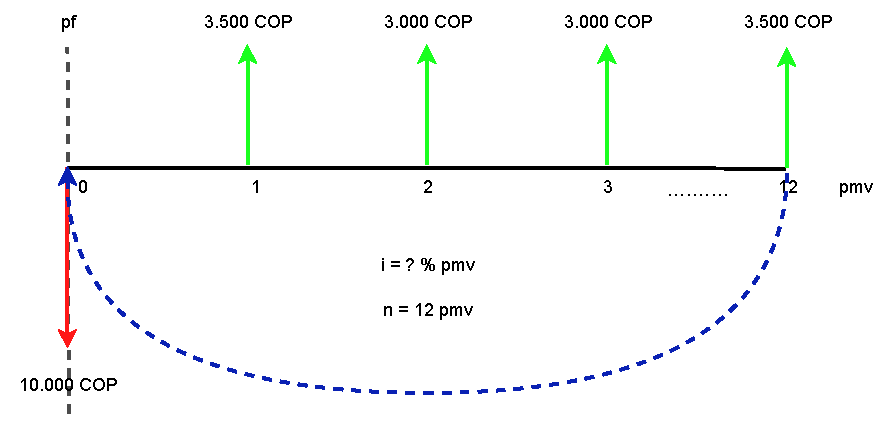
\includegraphics[scale=0.8]{ejemplos/5/Graf2Ej5Cap11.pdf} }
		\\
		\multicolumn{3}{|c|}{$ VPN(B-C)= -  10\text{.}000\text{ } COP +   3\text{.}500(1+i)^{-1}\text{ } COP + 3\text{.}000(1+i)^{-2}\text{ } COP  + $}
		\\
		\multicolumn{3}{|c|}{$  3\text{.}000(1+i)^{-3}\text{ } COP + 3\text{.}500(1+i)^{-4}\text{ } COP =   $ 0 $\text{ } COP$}
		\\
		\multicolumn{3}{|c|}{$ \text{TIRI = 11,41\% pmv, lo cual nos indica que el excedente de inversión (10.000 COP)} $}
		\\
		\multicolumn{3}{|c|}{$ \text{genera un interés del 1,41\% pmv que es inferior a la TMAR,}$}
		\\
		\multicolumn{3}{|c|}{$\text{ en consecuencia, el proyecto más costoso no es aconsejable por} $}
		\\
		\multicolumn{3}{|c|}{$ \text{ lo tanto nos quedamos con el proyecto C.} $}
		\\
		\multicolumn{3}{|c|}{$ \textbf{Se concluye así, que si B > A y C > B entonces C > B > A } $}
		\\
		\multicolumn{3}{|c|}{$ \textbf{ por lo tanto la decisión final es invertir en el proyecto C.} $}                    \\  \hline
		\multicolumn{3}{|c|}{$\text{Comprobación de la decisión usando el VPN usando la TMAR.}$}
		\\
		\multicolumn{3}{|c|}{$VPN(B)= $}
		\\
		\multicolumn{3}{|c|}{$ -  120\text{.}000\text{ } COP -  2\text{.}000(1+0.025)^{-1}\text{ } COP -  3\text{.}000(1+0.25)^{-2}\text{ } COP - $}
		\\
		\multicolumn{3}{|c|}{$ 4\text{.}000(1+0.25)^{-3}\text{ } COP - 5\text{.}000(1+0.25)^{-4}\text{ } COP$}
		\\
		\multicolumn{3}{|c|}{$ VPN(B)= -  127\text{.}616\text{ } COP $}
		\\
		\multicolumn{3}{|c|}{$ VPN(C)=  $}
		\\
		\multicolumn{3}{|c|}{$ -  110\text{.}000\text{ } COP - 5\text{.}500(1+0.025)^{-1}\text{ } COP - 6\text{.}000(1+0.25)^{-2}\text{ } COP - $}
		\\
		\multicolumn{3}{|c|}{$ 7\text{.}000(1+0.25)^{-3}\text{ } COP - 8\text{.}500(1+0.25)^{-4}\text{ } COP $}
		\\
		\multicolumn{3}{|c|}{$ VPN(C)=-  $ $ 125\text{.}306\text{ } COP $}
		\\
		\hline

		%%%%%%%%%% FIN MATEMÁTICAS
		%%%%%% FIN DESARROLLO MATEMÁTICO
		%%%%%% INICIO RESPUESTA
		\rowcolor[HTML]{FFB183}
		%%%%%%%%%%INICIO TITULO
		\multicolumn{3}{|c|}{\cellcolor[HTML]{FFB183}\textbf{6. Respuesta}}                                                 \\ \hline
		%%%%%%%%%% FIN TITULO
		%%%%%%%%%% INICIO RESPUESTA MATEMÁTICA

		\multicolumn{3}{|c|}{ \text{La mejor alternativa es el proyecto C,esto se puede comprobar porque el VPN de este proyecto}}
		\\
		\multicolumn{3}{|c|}{\text{es el mayor, la decisión es coincidente con la que indica la TIRI. } }
		\\
		\hline


		%%%%%%%%%% FIN MATEMÁTICAS
		%%%%%% FIN RESPUESTA
	\end{longtable}
	%Se crean dos lineas en blanco para que no quede el siguiente texto tan pegado
	%\newline \newline %USARLO SI CREES QUE ES NECESARIO
\end{center}
%%%%%%%%%%%%%%%%%%%%%%%%%%FIN EJERCICIO 1 %%%%%%%%%%%%%%%%%%%%%%%%%%%
